\documentclass[a4paper, 12pt, notitlepage]{report}

\usepackage{amsfonts} % if you want blackboard bold symbols e.g. for real numbers
\usepackage{graphicx} % if you want to include jpeg or pdf pictures
\usepackage{pdfpages}
\usepackage{url}
\usepackage{listings}

\title{Exam Invigilator Communications System\\
Interim Report} % change this
\author{Richard CB Evans\\
Department of Electrical and Electronic Engineering\\
Imperial College London} % change this
\date{\today} % change this

\begin{document}

\maketitle
\begin{center}
Supervised by Dr.\ Mark Wheelhouse. % change this
\end{center}
\thispagestyle{empty}
\newpage

\tableofcontents 

\chapter{Introduction}
%
Despite the high uptake of technology through the university education system, one aspect remains very manual: Exam Invigilation.

During each exam session, it is common to have invigilators spread across multiple rooms, either due to the popularity of certain courses, timetable collisions, or having students with extra time.

There are many reasons for which invigilators may need to communicate during these sessions.  For example, examination start and finish times need to be coordinated, clarifications or corrections need sharing amongst exam rooms, and students may need escorting to the bathroom.  This can be particularly troublesome for rooms with single invigilators.

Whilst most invigilators carry a mobile phone which could be used for communicating with other rooms, this is not a reliable solution to the communication issue.  Not all invigilators do carry a phone, and invigilators do not necessarily know the number of all other invigilators in other rooms.  Furthermore, it is necessary for all mobile phones to be placed in silent mode, leading to communications being missed.

Improving ease and speed of communication between exam invigilators is highly desirable as, ultimately, it will improve the quality of the student exam experience.  Quick and efficient communication will mean problems can be identified, shared and resolved more quickly, meaning students can receive corrections, visit the bathroom or obtain more paper sooner.  This allows the students to spend their time focussed on the task at hand; answering the paper in front of them.

The project is to create an easy to use and effective real-time communication system.

\chapter{Background}
%
In this chapter I will describe the background research done before any design or implementation decisions were made.

\section{System Requirements}

In this section I will describe the initial investigation done to establish the requirements of the system.

\subsection{Initial Research}

Before beginning development, it was essential to identify the requirements of the system additional to those outlined in the project specification.  Ultimately, the success of the system would be judged by those it was intended for; invigilators, and so I approached and interviewed an Imperial Department of Computing invigilator to establish the aspects of a prospective system which would influence his opinion of its success.

A number of areas were identified:

\begin{itemize}
\item Ease of Use\\
The interface must be simple enough to operate quickly and accurately.
\item Security\\
Examination information is often confidential and so access must be restricted to those  with the appropriate permissions.
\item Reliability\\
Exams are critical components of the university education process and so it is imperative that any computerised system would be completely reliable.  All information must be shared in real-time and shared with any and all necessary members of staff.  Any cause to resort to traditional communication methods would render the system a failure.
\item Discretion\\
The operation of the communication system must not disturb the students who are being examined in the room.  It is, however, important that the system be effective at drawing the users attention to any alerts and messages broadcast, to avoid information being missed.
\item Functionality\\
There are a certain number of functionalities which the system must offer to be considered useful to those invigilating:

\begin{itemize}
\item Show at a glance which room(s) need assistance.
\item Allow an invigilator to notify others when the exam(s) in their room have started or stopped.
\item Request an examiner come to their room, for example to answer a student's question.
\item Request assistance from another invigilator, for example to escort a student to the bathroom.
\item The requesting invigilator is able to see that someone is on the way to help, however, it is important that this information is shared such that a room is not over-serviced.
\item Broadcast an announcement to be made in all rooms of a certain exam, with acknowledgement of receipt.
\end{itemize}
\end{itemize}

\subsection{Further Research}

With the initial requirements discussed with an invigilator, I made the decision to reach out to other invigilators for more input with a short web survey which was shared via e-mail to the Department of Computing alias for all teaching fellows.  I also received interest from the Electrical and Electronic Engineering department and so shared the survey with the staff there to gather more opinions and information to assist with the direction the project should take.

The full results of the web survey can be found in appendix A.

\subsection{Research Results Analysis and Requirements}

In the online survey answered by the staff of both the Department of Computing and Electrical and Electronic Engineering, I asked a number of questions regarding the preference of device and feature specification.

By far the most prolific devices were phones running the Android operating system, owned by half of all respondents, followed by the iPhone, owned by 20\%.  iPhone combined with the iPad made up 9 devices owned by staff, with Android phones and tablets making 15.

When offered the choice of using an Android powered device, owned by the Department of Computing, or using their own device, 58\% of respondents indicated a preference of using a provided departmental device, however, when asked whether they would prefer the system to use a web interface or be a native application, 62\% indicated that they would prefer a web interface, with 12.5\% preferring a native application.

The preference for a web interface was discussed during the initial interview where, it was expressed that a native application running on a departmental tablet device would be best.  Whilst many invigilators take a laptop to exams, they generally spend the time working in full screen applications.  As a result, if a web interface were to be implemented for the system, they would likely have the system open in a background browser window while they work.  This would make any attempt at notifying of a message near impossible and would rely on them frequently checking the status of the system.  This would inconvenience them while they work, decreasing the likelihood of them checking regularly, making the system hard to justify.  Use of a tablet, however, would mean that extra functions such as a device vibrator and manipulation of the display could be used to attract attention of the invigilator and the device could also be left in a prominent position alongside them working to be seen.  This goes with the extra mobility of the device, allowing them to carry it whilst responding to students with raised hands, allowing them to advertise if assistance is needed instantly.  As a result, I have made the decision that an Android application should be the priority in development, with a web interface being a stretch goal that can be investigated if time permits as the project progresses.

The survey respondents were asked which information they felt it was important to have visible on the screen instantly accessible, and which functionality they felt would be important for a successful communication system.  The survey website attributed each response a value from 1-4 with increasing importance which was then divided by the number of respondents to give a response average value which the list could then be sorted by, as seen in the results tables in appendix A.  Respondents were further given the opportunity to give their own suggestions of functionality of notification methods.

\subsubsection{Core Functionality}

Having analysed the predetermined system requirements and the responses of all web survey respondents, the suggested features have been split into three functionality groups; the essential core functionality, and two stretch goal groups which can be attempted with sufficient time.  The system will be designed in such a way that inclusion of the stretch goal functionality will not require complete re-engineering of the core system.\\

Core Requirements:

\begin{itemize}
\item Allow Invigilators and Examiners to sign into the system and assign themselves to a specific room, or as floating staff

\item Provide the ability to update the room a user is in and reflect this change across the system

\item Offer a means of electronic text communication between invigilators and examiners
\begin{itemize}
\item Nature of Recipients
\begin{itemize}
\item Send to all
\item Send to all in specific room
\item Send to all examiners
\item Send to an individual
\end{itemize}
\item Nature of Message
\begin{itemize}
\item Preset generic assistance needed message
\item Preset specific assistance needed message, i.e. Bathroom Escort
\item Allow typing of custom messages
\end{itemize}
\item Acknowledgement of Message
\begin{itemize}
\item Provide a positive response to the individual requesting help
\item Dismiss notification on other users' screens so that the request is not over serviced
\item Append response to the communication log
\end{itemize}
\item Provide a log to browse the history of all communications
\end{itemize}

\item Allow users to view and control exam timings in their own room, and view the status of other rooms
\begin{itemize}
\item Exam start time
\item Time remaining
\item Exam finish time
\item Extra Time finish time
\end{itemize}

\item Provide a listing of active users on the system, and their locations.

\item Effectively alert users to new incoming messages in a way not distracting to students sitting the exam.

\end{itemize}

\subsubsection{Stretch Goals}

Beyond the core functionality specified above, the remaining ideas for functionality can be split into two categories of decreasing importance.  These requirements differ from the core list in that if not successfully implemented into the system, the system could be deemed a success as inter invigilator/examiner communication will be possible.

In the case that the project progresses in good time ahead of schedule, first group 1 then group 2 stretch goals will be implemented.

\begin{enumerate}
\item More Important
\begin{itemize}
\item Include information for each examination, including the examiner responsible for asking each question of a paper.
\item Include critical contact numbers for each exam paper.
\item Provide student seating plans mapping student names to numbers, and vice versa.
\item The ability to customize notification methods, e.g. Toggle device vibration on message received.
\end{itemize}

\item Less Important

\begin{itemize}
\item Implement a client web interface for the system.
\item Include additional information such as student ID photo in student list.
\item Add the ability to scan student IDs to automate up the ID checking process.
\item Use of the system to replace current pen and paper administration such as student count.
\end{itemize}
\end{enumerate}

\section{Available Data}

In the Department of Computing, all examination information and timetables, seating plans and invigilation schedules are already computerised and available via internal APIs.  This project will seek to build upon these available APIs to fetch and receive information as required, for example, to find the examiner for a specific question on a paper.

If it is found that the available APIs are incapable of providing adequate levels of detail necessary for the desired functionality of the system, I will engage with the Department to discuss the possibility of extending or improving the existing APIs, or investigate hosting information central to the Communication system which can then expose APIs for external use instead, if necessary.

\subsection{Confidentiality of Data}

As previously stated, the exam scheduling, seating plans and invigilator information contains sensitive data protected by the data protection act.  As a result, during the development of the system, I will make use of mock data.

\section{Existing Infrastructure}

\subsection{Server Hosting}
As it is necessary to centralise access to the existing APIs offering information about the exam timetables and other information, it will be necessary to make use of a server to which clients can connect and which hosts the information about ongoing exams.  Use a central server will also avoid complexities associated with peer to peer network discovery and communication.

CSG (Computer support group) at Imperial offer the cloudstack virtual server service which allows students to provision and administer their own virtual servers hosted on shared server hardware. The servers can be instantiated with a number of preconfigured template systems such as Ubuntu 12.04 and CentOS 6.4.

After the provisioning, the user has full root access to the server to customise as required.

\subsection{Network Communication}

The Department of Computing is already fitted with a widely accessible wireless local area network which interfaces the Virtual Cloud Server hosting.  Client server connection will therefore be possible via connection to the Imperial-WPA wifi connection, or via VPN from outside the college network.

\subsection{System Security}

Given the nature of the information to be made available in the exam invigilator communication system, it is necessary that the system features restricted access to only authorised members of the college faculty involved with the invigilation or examination of the papers.

Imperial offers two authentication services, LDAP (Lightweight Directory Access Protocol) Active Directory which supports single signon via Kerberos.  Having discussed with the college ICT Service Desk, it will be possible to make use of these authentication methods to authenticate client access to the system backend server.  It will be possible to create a system access alias against which any connecting clients can be checked.

The downside of this approach is that any invigilator or examiner must be added to this alias before the system will grant them access, however, this is unavoidable and much preferred to the overhead of implementing a security policy within the backend system itself.  ICT have indicated that given some criteria, it would be possible to create a policy rule which will automatically populate the user list from corporate data, keeping it up to date.

Kerberos and LDAP are widely supported authentication standards and so implementation of either with a major web server distribution should be highly feasible.

\section{Implementation Technologies}

In this section I will discuss the potential technologies which will be have been or will be investigated for use in the implementation of the system.

\subsection{Web Server}

Whilst I have previous experience with Apache web servers, a highly recommended implementation with good support for the websocket standard is Node.JS.  It has a number of high quality libraries quickly available for install using the node package manager, including libraries adding support for WebSockets such as socket.IO, a kerberos support library and all big database systems, MongoDB, CouchDB and various SQL implementations included.

Node.JS's event driven design and javascript based object oriented style makes it a very nice system to development with and so will be my web server of choice for this project.  If any major setbacks are experienced during the early stages of development I may reconsider this choice for an alternative such as Apache.

\subsection{Data Store}

There any many database software implementations with drivers available for Node.JS servers, both SQL and NoSQL.  Both SQL and noSQL implementations have their merits, but the great thing about noSQL is they work with objects as opposed to direct manipulation of data tables.  In JavaScript environments, such as with Node.JS this allows for easy data object traversal using natural JavaScript language such as shown in listing 2.1. 

\begin{minipage}{\textwidth}
\begin{lstlisting}[captionpos=b,caption=MongoDB Data Creation and Insertion, tabsize=2,
    breaklines=true]

// Retrieve
var MongoClient = require('mongodb').MongoClient;

// Connect to the db
MongoClient.connect("mongodb://localhost:27017/exampleDb", function(err, db) {
  if(err) { return console.dir(err); }

  var collection = db.collection('test');
  var doc1 = {'hello':'doc1'};
  var doc2 = {'hello':'doc2'};
  var lotsOfDocs = [{'hello':'doc3'}, {'hello':'doc4'}];

  collection.insert(doc1);

  collection.insert(doc2, {w:1}, function(err, result) {});

  collection.insert(lotsOfDocs, {w:1}, function(err, result) {});

});

\end{lstlisting}
\end{minipage}

Since the APIs providing data from the existing college systems (will eventually) provide their results in JSON format, the mongoDB document format for data is a perfect fit for purpose.  For this reason MongoDB shall be my database implementation of choice for this project unless, as with the choice of web server, any major setbacks are experienced.  Unlike migrating web server, the switch to an alternative database implementation should prove less troublesome.

Given the document driven nature of MongoDB I intend to investigate implementation of the base data for the system using a number of documents using a number collections, each containing a document for the given collection base type.  For example, in JSON style format:

\begin{minipage}{\textwidth}
\begin{lstlisting}[captionpos=b,caption=Example MongoDB Storage Structure for Exam information, tabsize=2,
    breaklines=true]

"Collection" : "exams",
"Documents" :
	{
		"528" : 
			{
				"name" : "Concurrent Programming",
				"date" : "2014-03-17",
				"sched_time" : "11:00:00",
				"duration" : "01:30:00",
				"extra_time" : "00:30:00",
				"rooms" : "144,145"
			},
		"C526" : 
			{
				...
			}
	}

\end{lstlisting}
\end{minipage}

A similar style can be implemented for seating plans and any other data that it is decided is needed.  This will work incredibly well if the DoC APIs do indeed provide JSON as is desired, however, even if it is not, it would be feasible to write a wrapper around the API call to convert the returned data to the required JSON format for storage.

\subsection{Network Application Layer Protocols}

WebSocket was developed as part of the HTML5 initiative and introduced the WebSocket JavaScript interface, defining a full-duplex single socket connection over which messages can be sent between client and server.

HTTP was designed as a request/response protocol bringing great complexities in cases where bi-directional communication was required.  The protocol was designed such that a client sends a request to the server and when and only when the request has been completely received, the server sends its response. As a result there are many techniques, or some may say 'hacks'\cite{httpabuse}, which have been employed to provide the illusion of full-duplex communication between client and server such as long-polling using AJAX\cite{lpAjax}.

WebSocket is purposefully designed to provide the functionality designed by modern real-time web applications and so makes perfect sense for use in this project.

By design, WebSocket is designed with a subscription model.  Any clients connecting subscribe to the Socket and the WebSocket server simply re-emits any received messages to all users.  This is not optimal behaviour though as in some cases, such as when a message has a specific intended recipient, bandwidth is wasted in transmitting to all users.  This is not disasterous as it is possible to simply process the received message payload on the client device and establish in the client-side software if the current device is the intended recipient.

I intend to implement a system where upon connection a user is assigned an ID in a hashmap structure of usernames and websocket connections and make use of my own JSON based API to communicate between devices.  JSON is fully supported in both Java, for the client application, and in JavaScript apps running on Node.JS, and so information can be encoded and parsed by both clients and server to establish the nature of the transmitted message.

An initial design for an API is as shown in listing 2.3.

\begin{minipage}{\textwidth}
\begin{lstlisting}[captionpos=b,caption=Proposed WebSocket API for System Communication, tabsize=2, breaklines=true]

{
    "type" : "message",
    "payload" : {
        "to" : "someone",
        "message" : {
          "from" : "me",
          "message_type" : "request",
          "message" : "A Student needs the bathroom"
        }
    }
}
\end{lstlisting}
\end{minipage}

With this API the server can parse the received message and check the message type.  This could be a message, a first contact (to establish username for the sending socket with the server), a request for application data such as rooms, exams etc.  The extensible nature of a JSON style API means extension of the API to support new message types is incredibly simple.  The payload of the message can then be processed, in this case, the "message" element of the payload will be forwarded to the intended recipient, identified by the "to" value.

\section{Initial Design Concept}

In this section I will show initial implementation design proposals for both the system as a whole, and the GUI of the Android client application.

\subsection{System Block Diagram}

\includegraphics[width=\textwidth]{"System Diagram/System Block Diagram"}

\subsection{Android Client GUI}

For and Android client GUI concept designs I decided to use a traditional pen and paper rapid prototype methodology.  By using pen and paper I was able to focus more on the general design of the application rather than beautifying or concentrating on details.

The client application designs are based upon the screen size and resolution of a Google Nexus 7 tablet and are drawn to scale.  Since the department of computing is already in possession of primarily tablets, this is the form factor I will be primarily designing for.  The code will be implemented using Android fragments\cite{fragments} such that, if there is sufficient time, it should be a relatively trivial task to create a usable layout design for phone form factors.  To simplify development, the application will also enforce landscape device rotation.

\includegraphics[width=\textwidth]{"GUI Sketches/Main Overview Cropped"}

The main overview page for the application will consist of a dual pane android layout using fragments.  2/3 of the screen will be dedicated to overview information, with the remaining 1/3 containing the log of most recent system communication activity.

The main overview content will be divided again roughly in two.  The top panel will contain a horizontally scrollable list of the rooms currently containing examinations, the invigilators/examiners currently linked to that room, and the rooms status; ok, stopped, or pending help, along with a traffic light icon reflecting the status.  The rooms are selectable, shown by highlighting which updates the information shown in the lower panel.

The initial concept for the lower panel of the main overview content is that it will contain another horizontally scrollable panel containing an entry for each exam taking place in that room.  Each entry will show the name of the room, and timing information depending upon the state of the exam.  Before the exam is started, the scheduled start time will be shown, with this changing to show the actual start time, time remaining, finish time, and extra time finish time.  If an exams time is extended, this can be reflected also, by appending an extra time flag to the finish time, for example

\begin{minipage}{\textwidth}
\begin{lstlisting}[captionpos=b,caption=Representation of Examination Timings, tabsize=4, breaklines=true]

 12:01							 12:02
  1:35			becomes			  1:44
 14:01							 14:11 (+0:10)
(14:31)							(14:41)(+0:10)

\end{lstlisting}
\end{minipage}

The exact method of enhanced functionality, such as how to extend the time of an exam for example are yet to be decided pending evaluation of the initial concept sketches.

\includegraphics[width=\textwidth]{"GUI Sketches/Side Menu View Cropped"}

The client application will feature an always available side bar menu available to the left hand side of the screen.  This will contain the navigation buttons to move to different activities within the android application.

The slide in menu may be implemented using either the inbuilt Navigation Drawer\cite{navdrawer} or using a third party library such as slidingPaneLayout\cite{spl}.  The main differences between these two implementation techniques are that the android Navigation Drawer overlaps the screen content, leaving the log visible at all times, whereas with the SlidingPaneLayout, it would be possible to achieve the effect shown in the sketch where the log is slid off the right side of the screen, with the menu taking up the left 1/3 of the screen.

\includegraphics[width=\textwidth]{"GUI Sketches/Help Request Window Cropped"}

The request help screen will allow the user to send a message requesting assistance to other users on the system.  They will be able to select send to all, send to examiners or send to specific users, with send to all the default choice.  They can then select the nature of the message whether it is a generic assistance needed message, a preset advanced message such as request for more paper or a toilet escort, or a manually typed specific message.

\includegraphics[width=\textwidth]{"GUI Sketches/Message Notification Cropped"}

Received messages when received by the client will be buffered for notification purposes.  One at a time a notification will be displayed on screen and the device will optionally vibrate to alert the user.  The message and the sender will be displayed, along with a time stamp.

The alert window will feature a number of responses which the user can make use of which will vary by nature of the alert being displayed.  The user can optionally choose to dismiss the message with no action being taken, in which case no response will be sent to the sender except for announcement requests, in which case even if dismissed the sender will be notified that the message has been seen.  If an announcement is positively responded to, such as by saying that the user is on their way to help, the message will be dismissed or removed from the queue on all other devices to prevent over servicing of requests.

\includegraphics[width=\textwidth]{"GUI Sketches/Seating Plan Cropped"}

The seating plan part of the system will allow a user to view the seating plan for a selected room giving the student names, CID (College ID) numbers and seat numbers.  This list will be sortable by name or by seat number and there will be a search functionality for looking up seating positions based on name/CID or a reverse lookup to identify missing students based on seat number.

\chapter{Project Plan}
%

The project is split into five main phases; investigative, implementation phases 1, 2, 3 and evaluation.

I have already completed a large majority of the investigative phase where I establish the requirements of the system.

This plan is shown in figure 3.1.  The plan is largely linear as since I am working on my own, my ability to implement multiple tasks in parallel is somewhat limited.  I have therefore made an assumption that I can only work on one thing at a time.  I can dynamically adjust my schedule to change the order of task implementation, for example switching to something else if I reach a point where I am making little progress on a task and need a break.

\begin{figure}[h]
\begin{center}
\begin{minipage}{1.4\textwidth}

\hspace{-1.1in}
\centerline{\includegraphics[width=\textwidth]{"Project Plan/PP"}}

\end{minipage}
\end{center}
\caption{Project Plan for ExICS}
\end{figure}

\chapter{Evaluation Plan}
%

\appendix
\chapter{Web Survey Results}

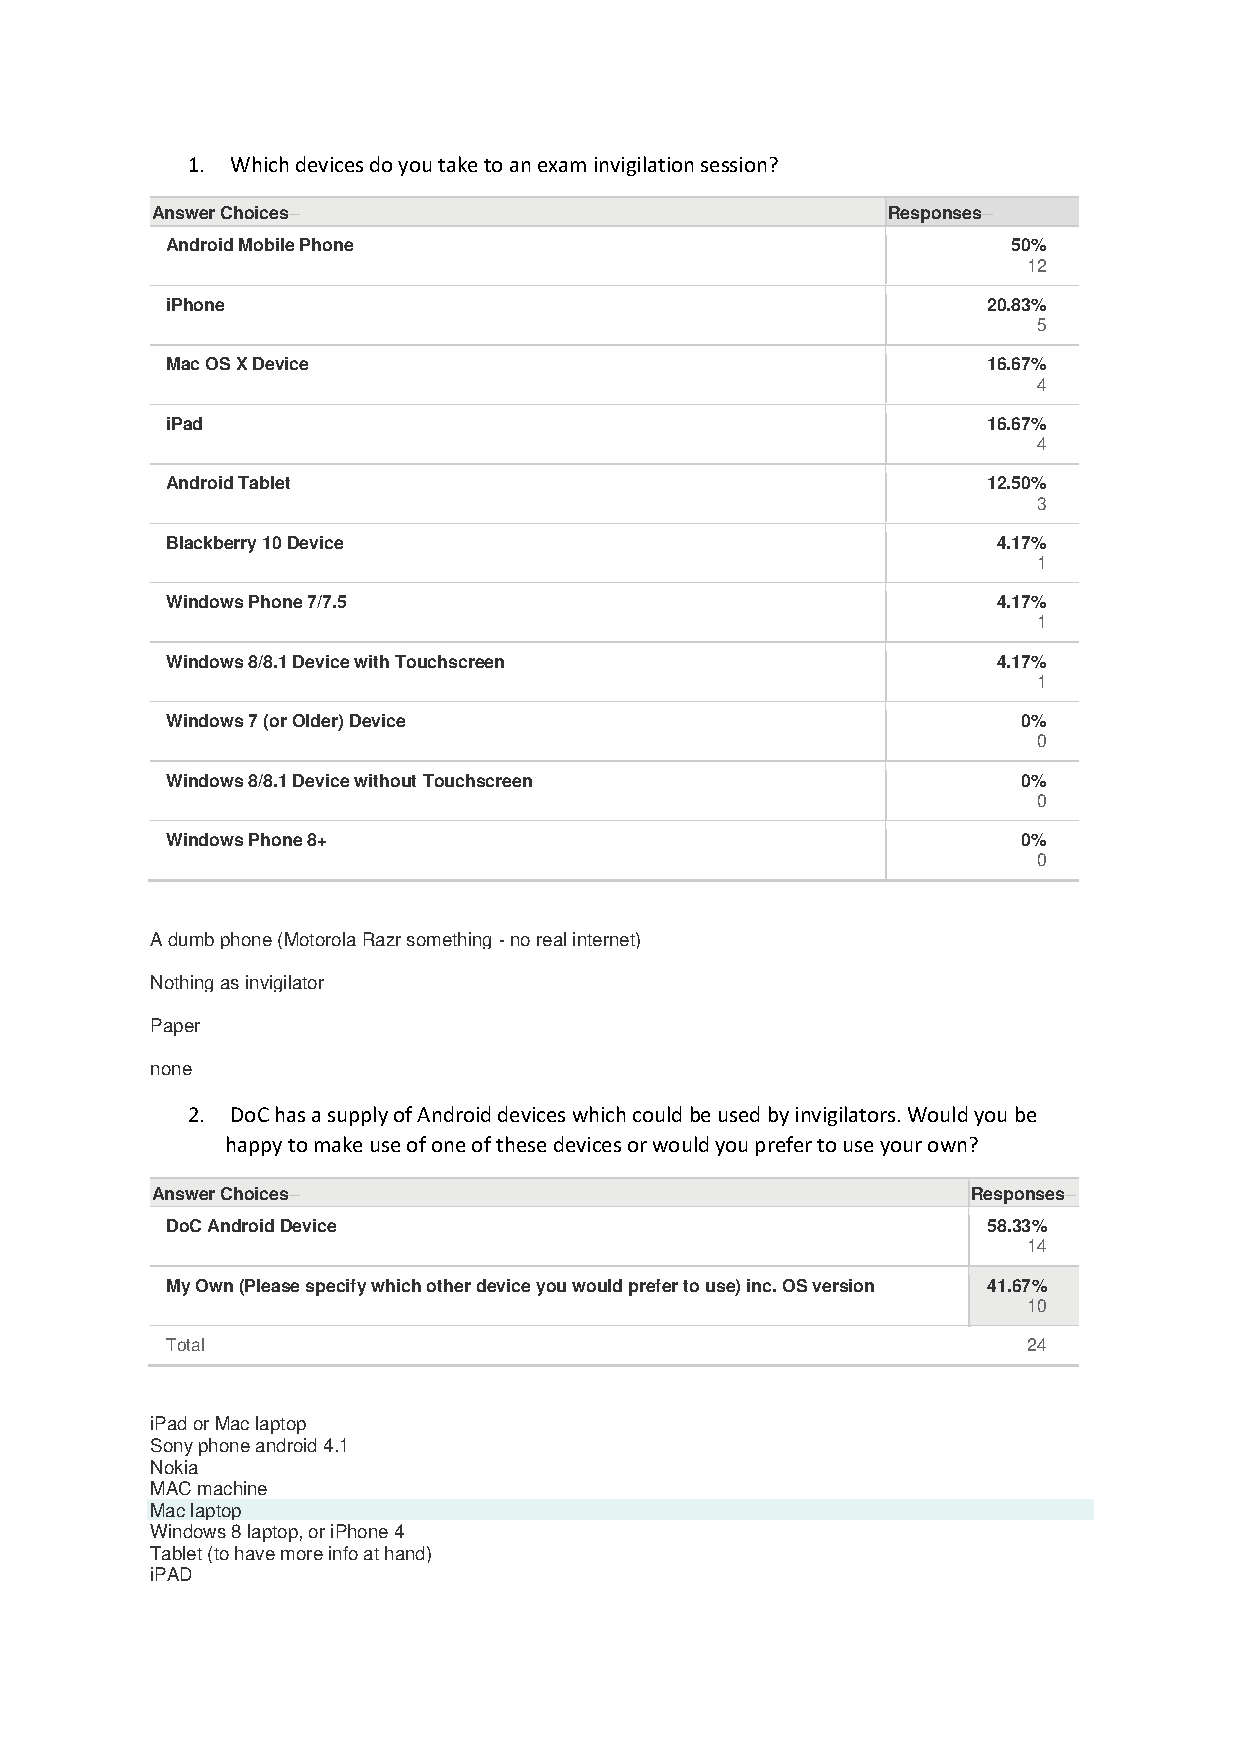
\includepdf[pages=-]{surveyResult.pdf}

\bibliographystyle{plain}
\bibliography{ref}

\end{document}